\documentclass{problems}


\title{Problems of dynamics of structures}
\author{J. Bonet, M. Masó, R. Chacón}


\begin{document}

\maketitle

\section{Free vibration of SDOF structures}

\problem{1}
For the structures shown, determine the natural frequency of vibration using simple structural concepts.

\begin{center}
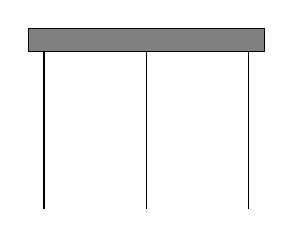
\begin{tikzpicture}
    \draw[fill=gray] (0,2) rectangle (3,2.3);
    \draw (0.2,0) -- (0.2,2);
    \draw (1.5,0) -- (1.5,2);
    \draw (2.8,0) -- (2.8,2);
\end{tikzpicture}
\hfill
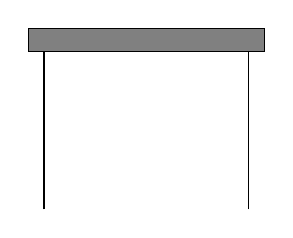
\begin{tikzpicture}
    \draw[fill=gray] (0,2) rectangle (3,2.3);
    \draw (0.2,0) -- (0.2,2);
    \draw (2.8,0) -- (2.8,2);
\end{tikzpicture}
\hfill
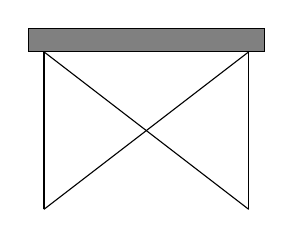
\begin{tikzpicture}
    \draw[fill=gray] (0,2) rectangle (3,2.3);
    \draw (0.2,0) -- (0.2,2);
    \draw (2.8,0) -- (2.8,2);
    \draw (0.2,0) -- (2.8,2);
    \draw (0.2,2) -- (2.8,0);
\end{tikzpicture}
\end{center}



\problem{2}
For the structures shown, determine the natural frequency of vibration using Rayleigh's method.



\section{Forced vibration of SDOF structures}


\problem{5}

\section{Vibration of MDOF structures}


\section{Solutions}

\end{document}
